\section{\I{The population section}\label{sec:population-section}}

\subsection{Introduction}

The population section\index{Population section} specifies the model structure, movement and population dynamics, and other associated parameters. It describes the model structure (both the spatial and population structure), defines the population  (for example, recruitment, migration, and mortality) and movement processes, defines the layers (the known attributes of each spatial cell), selectivities, and model parameters.

The population section consists of several components, including;
\begin{itemize}
  \item The spatial and population structure
  \item Model initialisation (i.e., the state of the model at the start of the first year)\index{Initialisation}\index{Model ! initialisation}
  \item The years over which the model runs (i.e., the start and end years of the model)
  \item The annual cycle (time-steps and processes that are applied in each time-step)\index{Annual cycle}
  \item The specifications and parameters of the processes;
  \begin{itemize}
    \item Population processes (i.e., processes that add, remove individuals to or from the partition, or shift numbers between ages and categories in the partition)
    \item Spatial processes (i.e., processes that move or shift cohorts between spatial locations but do not alter their ages or categories)
  \end{itemize}
  \item Layers (used by processes, observations and reports) and their definitions
  \item Selectivities
  \item Parameter values and their definitions
  \item Derived quantities, quantities by cell and meta-layers required as parameters for some processes (i.e., spawning stock biomass to resolve the spawner-recruit relationship in a recruitment process)
\end{itemize}

\subsection{\I{Spatial structure}\label{sec:spatial-structure}}

The spatial structure of \SPM\ is represented by an $n_{rows} \times n_{cols}$ grid, with rows $i=1 \dots n_{rows}$ and columns $j=1 \ldots n_{cols}$. Each cell of this matrix records the population structure at that point in space, where the population structure is represented by an $n_{categories} \times n_{ages}$ rectangular matrix (with categories $k=1 \ldots n_{categories}$ and ages $l=1 \ldots n_{ages} = age_{min} \ldots age_{max}$. Hence we can describe any spatial and population element of the model as element$(i,j,k,l)$. We define, within the spatial grid ($n_{rows} \times n_{cols}$), locations where the population can and cannot potentially be present using a \emph{layer}. 

\SPM\ implements a single spatial structure, a grid of \emph{square} cells (Figure \ref{fig:SquareSpatialStructure}). The spatial grid can be of an arbitrary size, but must be rectangular. 

The dimensions of the spatial grid are user defined but must be at least a $1 \times 1$ grid (i.e., a single spatial cell), and the largest spatial structure currently allowed by \SPM\ is a grid of $1000 \times 1000$ cells\index{Maximum size of the spatial grid} -- although we note that models of this size are untested and will probably have very long run times. 

Associated with the $n_{rows} \times n_{cols}$ spatial structure is the one compulsory layer (see Section \ref{sec:layers}), the \emph{base layer}\index{Base layer}. This defines the locations where the population can and cannot potentially be present (e.g., in a marine model, the locations associated with the sea and not land). These are defined as the cells where the base layer has a value greater than zero. There must be at least one cell in the spatial grid where the population can be present. In addition, the base layer also defines the relative \emph{area}\index{Cell area} of each spatial cell that is used for density calculations within \SPM.

\begin{figure}[htp]
 \centering
	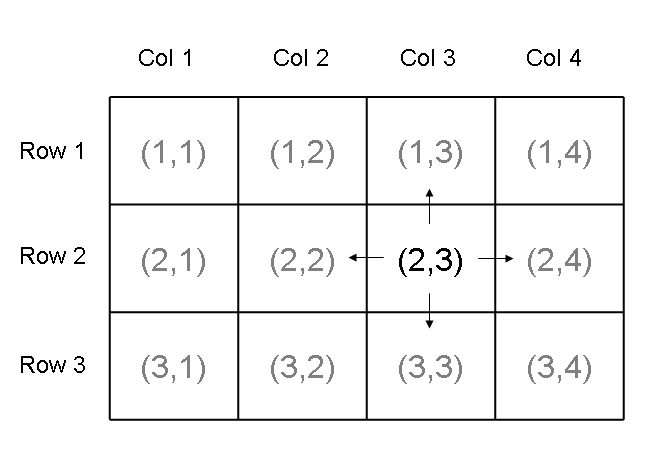
\includegraphics[width=0.66\textwidth]{Figures/SquareStructure}
  \caption{An illustration of the spatial structure}
  \label{fig:SquareSpatialStructure}
\end{figure}

Models are implemented as a grid of square cells making up a rectangular matrix. Distance between cells is determined as the euclidean\index{Inter-cell distance} distance between cell centres, modified by an arbitrary scalar. 

Hence, the definition of the spatial structure includes;
\begin{itemize}
\item The type of spatial grid and its dimensions, $n_{rows}$ and $n_{cols}$
\item The label of a numeric layer to be used as the base layer (defining the locations where the population can be present as well as the area of each cell)
\item The length (distance) of a side of the grid cell to be used as the scaler for distance calculations
\end{itemize}

\subsection{\I{Population structure}}

The population structure in \SPM\ is represented by a matrix containing an arbitrary number of user defined categories (rows), and an arbitrary age range (columns). Hence, each spatial cell has a population state described as $n_{categories} \times n_{ages}$ rectangular matrix with categories $k=1 \ldots n_{categories}$ and ages $l=age_{min} \ldots age_{max}$. 

The names and number of categories are user defined, but there must be at least one category defined for a model. The ages are defined as a sequence from $age_{min}$ to $age_{max}$, with the last age optionally a plus group. In order to calculate biomass, the age-size relationship for each category must also be defined.

Hence, the definition of the population structure includes;
\begin{itemize}
  \item The number and labels of the categories, $k_{categories}$
	\item The age\_size relationship for each category
  \item The minimum and maximum ages that define the ages of the model, $l_{ages}$
  \item If the last age is a plus group
\end{itemize}

\subsection{\I{Layers}\label{sec:layers}}

Layers are a key underlying concept in \SPM. They comprise of a grid of known values, with a value for every spatial cell in the model. Layers are used by processes, observations, and outputs commands to supply spatially explicit covariates and any categorical groupings required. 

\emph{Layers} are used by \SPM\ to evaluate locations where the population may be present (via the \emph{base layer}), to provide sets of known attributes or values of each spatial location (for some processes and for preference based movements), and to group or categorise cells for use by processes and observations. Layers consist of an $n_{rows} \times n_{cols}$ matrix and can be either \emph{numeric} or \emph{categorical}. 

Every model must define at least one layer, the base layer $L_B$. A layer is defined as a $n_{rows} \times n_{cols}$ matrix of values (albeit with one exception --- the distance layer --- which we describe below), where the value in each cell represents a known quantity. For example layers may represent classifications, physical attributes, or some other known or assumed quantity. Typically they are provided by the user as a matrix of values, although some layer (e.g., abundance and distance layers) can be calculated by \SPM\ during a model run. 

Within \SPM, layers are used in the following contexts:
\begin{enumerate}
\item The base layer\index{Base layer}\index{Layers ! the base layer}: The base layer $L_B$ is a special layer (there must be exactly one base layer defined within the model) that defines the locations where the population can and cannot potentially be present (e.g., locations associated with the sea and not land in a marine model). Here, we define that a cell may potentially have part of the population present if every element $L_B(i,j) \ge 0$. Further, positive values of the base layer $L_B$ represent the \emph{area} represented by that spatial cell. Note, the values in the base layer must be numeric, but cannot be a meta-layer (\emph{see below}).
\item \I{Covariate layers}: A model may have many covariate layers, and these are used as covariates of some population or movement process (e.g., the sea floor depth may be a covariate of some movement process). The values in layers used as covariates can be either numeric or categorical.
\item \I{Classification layers}: A model may have many classification layers, and these are used as a classification or grouping variable for aggregating data over individual spatial cells $(i,j)$, e.g., statistical areas or management areas. Such layers are typically used to aggregate the population within cells into groups so-as to allow comparison with observations. The values in layers used as classification layers must be categorical.
\end{enumerate}

\SPM\ defines the following types of layer;

\begin{enumerate}
\item{\I{Numeric layers}\label{numeric-layer}}: A model may have many numeric layers, and these can be used as covariates of a population or movement process (e.g., depth may be a covariate of some movement process), and/or locations of event mortality. Numeric layers can contain only continuous (numeric) variables. Values for a numeric layer must be supplied for each cell by the user. Numeric layers can be rescaled to sum to some user-defined value, and unlike other layers, the values for each cell can be estimated. 

\item {\I{Categorical layers}\label{categorical-layer}}: A model may have many categorical layers, and these can be used as a classification or grouping variable for aggregating data over individual cells, e.g., management areas; or as covariates of a population or movement process. Such layers are typically used to aggregate the population within cells into groups for comparing with observations, or to apply specific movement characteristics. The values in layers used as categorical layers can contain any characters (except white space), and are interpreted as categorical values. Values for a categorical layer must be supplied for each cell by the user.

\item {\I{Distance layers}}: A distance layer is one that defines the distance between any two cells. By default, \SPM\ calculates the values of the distance layer as the Euclidean distance. Here, the distance between cell $a$ and cell $b$ can be defined as,
\begin{equation}
  d(a,b) = \lambda \sqrt{(x_a - x_b)^2 + (y_a - y_b)^2}
\end{equation}
where $x$ and $y$ represent the x- and y-coordinates of $a$ and $b$ respectively, and $\lambda$ is an arbitrary scaler representing the length of one side of the square. Unlike other types of layers, distance layers are not a $n_{rows} \times n_{cols}$ grid of values, but rather a matrix of dimension $(n_{rows} \times n_{cols}) \times (n_{rows} \times n_{cols})$  where the distance between each cell and every other cell is evaluated. Note that under this definition, the distance between any cell and itself is 0. 

For example, to specify a distance layer, use,

{\small{\begin{verbatim}
@layer Distance
type distance
\end{verbatim}}}

\item{\I{Abundance layers}}: The abundance layer is the sum of the number of individuals within cell $a$ in categories $k$ and with selectivity $S_l$ at age $l$. 
\begin{equation}
  N(a) = \sum\limits_{k} \sum\limits_l S_l \ \text{element}(i,j,k,l)
\end{equation}
\SPM\ calculates the values of the layer when running the model at the point in time where the value is required.

For example, to specify an abundance layer of all individuals who are categorised as \texttt{mature}, use,

{\small{\begin{verbatim}
@layer Abundance
type abundance
categories mature
selectivities One
\end{verbatim}}}

\item {\I{Biomass layers}}: The biomass layer is the sum of the biomass of individuals within cell $a$ in categories $k$, with selectivity $S_l$ at age $l$, and mean weight $w_{kl}$
\begin{equation}
  N(a) = \sum\limits_{k} \sum\limits_l w_{k,l} S_l \ \text{element}(i,j,k,l) 
\end{equation}
\SPM\ calculates the values of the layer when running the model at the point in time where the value is required.

For example, to specify a biomass layer of all individuals who are categorised as \texttt{mature}, use,

{\small{\begin{verbatim}
@layer Biomass
type biomass
categories mature
selectivities One
\end{verbatim}}}

\item {\I{Abundance-density layers}}: The abundance density layer is the density of the number of individuals within cell $a$ with area $A_a$ in categories $k$, with selectivity $S_l$ at age $l$,
\begin{equation}
  N(a) = \frac{1}{A_a} \sum\limits_{k} \sum\limits_l S_l \ \text{element}(i,j,k,l)
\end{equation}
\SPM\ calculates the values of the layer when running the model at the point in time where the value is required.

For example, to specify an abundance density layer of all individuals who are categorised as \texttt{mature}, use,

{\small{\begin{verbatim}
@layer AbundanceDensity
type abundance_density
categories mature
selectivities One
\end{verbatim}}}

\item {\I{Biomass-density layers}}: The biomass-density layer is the density of the biomass of individuals within cell $a$ with area $A_a$ in categories $k$, with selectivity $S_l$ at age $l$, and mean weight $w_{kl}$,
\begin{equation}
  N(a) = \frac{1}{A_a} \sum\limits_{k} \sum\limits_l w_{k,l} S_l \ \text{element}(i,j,k,l)
\end{equation}
\SPM\ calculates the values of the layer when running the model at the point in time where the value is required.

For example, to specify a biomass density layer of all individuals who are categorised as \texttt{mature}, use,

{\small{\begin{verbatim}
@layer BiomassDensity
type bioomass_density
categories mature
selectivities One
\end{verbatim}}}

\item {Derived quantity and derived quantity by cell layers}\label{derived quantity layer}\index{Derived quantity layers}\index{Derived quantity by cell layers}: \SPM\ can use values from a derived quantity or a derived quantity by cell as a layer. These are the values of a derived quantity, and require an offset (in years) to extract the desired value for each year. They will extract the derived quantity either for each cell (for derived quantities by cell) or as a total value applied to each cell (for ordinary derived quantities) as values for a layer.

For example, to specify a layer of the biomass of all individuals who are categorised as \texttt{mature} in time step \texttt{StepOne} from two years ago, first define a derived quantity,

{\small{\begin{verbatim}
@derived_quantity_by_cell Mature
type biomass
categories mature
selectivities One
time_step StepOne
\end{verbatim}}}

Then define the derived layer,

{\small{\begin{verbatim}
@layer MatureBiomass
type derived_quantity
derived_quantity Mature
year_offset 2
\end{verbatim}}}

\item {\I{Meta-layers}\label{meta-layers}}: \SPM\ defines a special type of layer known as a \emph{meta-layer}. Meta-layers allows individual layers to be indexed by year and applied as an annually varying layer within the model. For example, assume a model that uses Sea Surface Temperature (SST) as a layer, perhaps to drive some movement process. The SST values for each year of the model would be defined as individual layers, each with a unique label. A meta-layer could be defined that indexed the individual annual SST layers by year, and used as a covariate layer in the movement process. Meta-layers have a \emph{default} layer that is used for time periods that are not specifically defined. Meta layers can be used wherever ordinary layers are used (except as  the base layer), with \SPM\ extracting the appropriate layer value corresponding to the year or initialisation phase.

\begin{enumerate}

\item {\I{Numeric meta-layers}\label{numeric meta-layer}}: Numeric meta-layers are a meta layer of numeric layers --- the individual ordinary layers that make up the meta-layer must all be of numeric type. For example, to specify a numeric meta-layer with specific values for the years 1990-1995, and a default for all other years (including the initialisation phases), use, 

{\small{\begin{verbatim}
@layer AnnualLayer
type meta-layer
default_layer SST
years    1990    1991    1992    1993    1994    1995
layer SST1990 SST1991 SST1992 SST1993 SST1994 SST1995
\end{verbatim}}}


\item {\I{Categorical meta-layers}\label{categorical meta-layer}}: Categorical meta-layers are a meta layer of categorical layers --- the individual ordinary layers that make up the meta-layer must all be of categorical type. Categorical meta-layers are specified in the same way as numeric meta-layers.

\end{enumerate}
\end{enumerate}

\subsection{\I{Time sequences}}

The time sequence of the model is defined in two parts;
\begin{itemize}
  \item \I{Initialisation}
  \item \I{Run years}
  %\item \I{Projection year}s
\end{itemize}

\subsubsection{\I{Annual cycle}}

The annual cycle is implemented as a set of processes that occur, in a user-defined order, within each year. time-steps are used to break the annual cycle into separate components, and allow observations to be associated with different sets of processes. Any number of processes can occur within each time-step, in any order and can occur multiple times within each time-step. Note that time-steps are not implemented during the initialisation phases (effectively, there is only one time-step), and that the annual cycle in the initialisation phases can be different from that which is applied during the model years.

\subsubsection{\I{Initialisation}}

Model initialisation can occur in several phases\index{Initialisation!phases}, each which iterates through a number of years carrying out the population and/or spatial processes defined for that phase. At the end of the initialisation step, \SPM\ runs through the model years carrying out processes in the order defined in the annual cycle, and can evaluate expected values of observations in order to calculate likelihoods, %project forward to determine future states \NYI, 
or simulate observations from the current state.

\SPM\ initialises the initial equilibrium state as an iterative process: a general solution that initialises complex structured movement models can be difficult to implement using analytic techniques. However, initialising via iteration for a long-lived species with complex movements can take many iterations and be slow to run. In \SPM, we allow for user-defined multi-phased initialisation using iteration to allow the user to optimize models for speed. Each phase of the initialisation can involve any number of population and/or movement processes. Note that the length of the initialisation period may affect the model outputs, and that a period should be chosen to allow the population state to converge.

In addition, each initialisation process can optionally be stopped early if a user defined convergence criteria is met. For a set of user defined years in the initialisation phase, convergence is defined as met if the proportional absolute summed difference between the the state in year $t-1$ and the state in year $t$ ($\widehat{\lambda}$) is less than $\lambda$ where, 
\begin{equation}
  \widehat{\lambda} = \frac{\sum\limits_{i} \sum\limits_{j} \sum\limits_{k} \sum\limits_l \left|\text{element}(i,j,k,l)_t - \text{element}(i,j,k,l)_{t-1} \right|}{\sum\limits_{i} \sum\limits_{j} \sum\limits_{k} \sum\limits_l \frac{}{}\text{element}(i,j,k,l)_t}
\end{equation}

In each initialisation phase, the processes defined for that phase are carried out and used as the starting point for the following phase or, if it is the last phase, then the years that the model is run over. The first phase is always initialised with each element (i.e., each age and category within each spatial cell) set at zero. Note that this means that recruitment processes where the numbers of recruits is based on a stock recruitment or density dependant relationship will likely fail if used in the first phase of an initialisation. 

The multi-phase iteration\index{Multi-phase iteration} also allows the user to determine if the initialisation has converged in a particular model run. Here, add an additional initialisation phase for, say, $1$ year as the last initialisation phase (with the same processes applied). Then, using the initialisation reports (\commandlabsubarg{report}{type}{initialisation\_phase}), print a copy of the partition just before and just after that phase. If the initialisation has converged to an equilibrium state, then the partition at both these time intervals will be the same.

Hence, for initialisation you need to define;
\begin{itemize}
  \item The initialisation phases
  \item The number of years in each phase and the processes to apply in each
\end{itemize}

\subsubsection{\I{Model years}}

Following initialisation, the model then runs over a number of user-defined years. For this part of the model, the annual cycle can be broken into separate time-steps, and observations can be associated with the state of the model at the end of any time-step, i.e., likelihoods for particular observations are evaluated, if required, at the end of each time-step. 

Processes are carried out in the order specified within each time-step, and can be the same or different to processes in other initialisation phases of the model. The run years define the years over which the model is to run and the annual cycle within each year. The model runs from the start of year \argument{initial} and runs to the end of year \argument{current}. %The projection part then extends the run time up to the end of year \argument{final}. 

\begin{itemize}
  \item The time-steps and the processes applied in each
  \item The initial year (i.e., the model start year)
  \item The current year (i.e., the model end year)
  %\item The final year (i.e., the model projection end year)
\end{itemize}

%\subsubsection{\I{Projections}\label{sec:projections}}
%
%\SPM\ can project, from a set of parameter estimates, the state of the model into the future \NYI. In a projection run, the model is initialised and run through the model years from \argument{initial} to the \argument{current}. Then, the model is run from \argument{current} to \argument{final}. 

\subsection{\I{Processes}}

Processes produce changes in the model partition, by adding, removing or moving individuals between spatial cells (movement processes), and ages or categories (population processes). These include processes such as recruitment, mortality, ageing, and various forms of movement.

\SPM\ has two types of processes, \emph{population}\index{Population processes} and \emph{movement}\index{Movement processes} processes. Population processes are those processes which modify, move or otherwise change the numbers of individuals \emph{within} a spatial cell, i.e., they do not affect the spatial location of a cohort. Movement processes, on the other hand, move, shift or otherwise modify cohorts \emph{between} spatial cells, but do not affect the age or category of the numbers in each cohort. 

The population processes include recruitment\index{Recruitment}, ageing\index{Ageing},  mortality\index{Mortality} events (e.g., natural and exploitation) and category transition processes\index{Category transition} (i.e., processes that move individuals between categories, while preserving their age structure). See Section \ref{sec:population-section} for a complete list of available processes.

Each of these processes is carried out in the user-defined prescribed order when initialising the model, and then for a user-defined order in each year in the annual cycle\index{Annual cycle}.

\SPM\ implements three different types of movement processes\index{Movement};
\begin{enumerate}
	\item  A migration movement rate\index{Migration}\index{Movement ! Migration} of cohorts between any two locations, and is roughly analogous to movements between areas as implemented in other population models, such as CASAL \citep{1388}. 
	\item An adjacent cell movements\index{Adjacent cell movement}\index{Movement ! Adjacent cell movement}, parametrised by some function of an underlying layer --- equivalent to, for example, movement processes implemented in Fish Heaven \citep{1136,1135}. 
	\item Movement parametrised as a probability density function\index{Preference movement}\index{Movement ! Preference movement}. Here, the key underlying idea is that the spatial distribution of cohorts at any point in time and at any location can be represented as a density function based on attributes of that location, local abundance, and/or distance from their previous location \citep{1366,1367}. 
\end{enumerate}

An \SPM\ model can be parametrised by both population processes (for example, ageing, recruitment, and mortality), and movement processes. Population processes are those processes which modify, move or otherwise change the numbers of individuals within a spatial cell, i.e., they do not affect the spatial location of a cohort. Movement processes, on the other hand, move, shift or otherwise modify cohorts between spatial cells, but do not affect the age or category of the numbers in each cohort. 

\subsection{\I{Population processes}}

Population processes are those processes that change the population state of individuals, but retain their location. The population processes are described below.

\subsubsection{\I{Recruitment}}

Recruitment processes are defined as  process that introduces new individuals into the model. \SPM\ implements four types of recruitment process, constant recruitment\index{Recruitment ! Constant},  \I{Beverton-Holt recruitment}\index{Recruitment ! Beverton-Holt} \citep{1203}, \I{local Beverton-Holt recruitment}\index{Recruitment ! Local Beverton-Holt}, and recruitment proportional to an abundance or biomass \index{Proportional recruitment}\index{Recruitment ! proportional}.

In the recruitment processes, the number of individuals are added to a single age class within the partition, with the amount defined by the type of recruitment process and its function. If more than one category is defined, then the proportion of recruiting individuals to be added to each category is specified by the \argument{proportions} parameter. For example, if recruiting to categories labelled male and female, then you might set the proportions as $0.5$ and $0.5$ respectively to denote that half of the recruits recruit to the male category and the remaining half to the female category.

Recruitment occurs in those cells defined by a layer, or all cells if a layer has not been specified.

For the constant, Beverton-Holt, and proportional recruitment processes, the  number of individuals in cell cell$(i,j)$ following recruitment in year $y$ is,  
\begin{equation}
  \text{element}(i,j,k,l) \leftarrow \text{element}(i,j,k,l) + p_k(R_y / n) \frac{L_ij}{\sum_ij L_ij}
\end{equation}

where age is the age defined as the recruitment age, $p_k$ is the proportion to category $k$ defined to have recruitment, $n$ is the number of spatial locations where recruitment occurs, and the recruitment to each cell is scaled to be proportional to the value of the layer in that cell. See below for how $R_y$ is determined in each of these cases.

In the local Beverton-Holt recruitment process, individuals are recruited to an individual cell, based on the local abundance or biomass (i.e., the local SSB). For each cell where cell$(i,j)$ is a member of some layer $L_R$, the number of individuals in that cell following recruitment in each year $y$ is 
\begin{equation}
  \text{element}(i,j,k,l) \leftarrow \text{element}(i,j,k,l) + p_k R_y L_{ij}
\end{equation}

where age is the age defined as the recruitment age, $p_k$ is the proportion recruitment to category $k$ defined to have recruitment, and the recruitment to each cell is the product of the Beverton-Holt stock recruitment relationship ($R_y$). 

\subsubsection*{\I{Constant Recruitment}}

In the constant recruitment process the total number of recruits added each year is $R_y$, and is simply $R_0$, i.e.,
\begin{equation}
  R_y = R_0
\end{equation}

It is equivalent to a Beverton-Holt recruitment process where steepness is set equal to one ($h=1$).

For example, to specify a constant recruitment process, where individuals are added to the category `immature' at $age=1$, and the number to add is $R_0=5 \times 10^5$ in areas proportional to the value of the layer \texttt{recruitment}, then the syntax is,

{\small{\begin{verbatim}
@process Recruitment
type constant_recruitment
categories immature
proportions 1.0
R0 500000
age 1
layer recruitment
\end{verbatim}}}

\subsubsection*{\I{Beverton-Holt recruitment}}

In the Beverton-Holt recruitment process the total number of recruits added each year is $R_y$, and is the product of the average recruitment $R_0$, the annual year class strength multiplier, $YCS$, and the stock-recruit relationship i.e.,
\begin{equation}
  R_y = R_0 \times YCS_{y-offset} \times SR(SSB_{y-offset})
\end{equation}
  
where $offset$ is the number of years offset to link the year class with the year of spawning $y$, and $SR$ is the Beverton-Holt stock-recruit relationship parametrised by the steepness $h$,
\begin{equation}
SR(SSB_y) = \frac{SSB_y}{B_0} / \left( 1-\frac{5h-1}{4h} \left( 1-\frac{SSB_y}{B_0} \right) \right)
\end{equation}

Note that the Beverton-Holt recruitment process requires a value for $B_0$ and $SSB_y$ to resolve the stock-recruitment relationship. Here, a derived quantity (see Section \ref{sec:derived-quantities}) must be defined that provides the annual $SSB_y$ for the recruitment process. $B_0$ is then defined as the value of the $SSB$ at the end of one of the initialisation phases. During initialisation the YSC multipliers are assumed to be equal to one, and recruitment that happens in the initialisation phases that occur before and during the phase when $B0$ is determined is assumed to have steepness $h=1$ (i.e. in those initialisation phases, recruitment is simply equal to $R_0$). Recruitment in the initialisation phases after the phase where $B_0$ was determined follow the Beverton-Holt stock-recruit relationship defined above. Recruits are then distributed across cells in proportion to the values in a numeric layer. 

For example, assume a Beverton-Holt recruitment process, where individuals are added to the category `immature' at $age=1$, the number to add is $R_0=5 \times 10^5$ in areas proportional to the value of the layer \texttt{MyRecruitment}. Then \texttt{SSB\_Biomass} is a derived quantity that specifies the total spawning stock biomass, with $B_0$ the value of the derived quantity at the end of the initialisation phase labelled \texttt{phase1}. The YCS are standardised to have mean one in the period 1994 to 2004, and recruits enter into the model two years following spawning. Then the command specification is,

{\small{\begin{verbatim}
@process Recruitment
type BH_recruitment
categories immature
proportions 1.0
R0 500000
steepness 0.75
age 1
layer MyRecruitment
B0 phase1
SSB SSB_Biomass
standardise_YCS_years 1994-2004
YCS_years 1994 1995 1996 1997 1998 1999 2000 2001 2002 2003 2004 2005 2006
YCS_values   1    1    1    1    1    1    1    1    1    1    1    1    1
SSB_offset 2
\end{verbatim}}}

Note that if not specified, $SSB\_offset$ is set at the value of $age$. This corresponds to cases where recruitment happens after spawning. $SSB\_offset$ can be user-defined to a different value if needed --- for example, if recruitment happens in a time-step before spawning, the offset will need to be specified as $age + 1$.

\subsubsection*{\I{Local Beverton-Holt recruitment}}

The local Beverton-Holt recruitment process assumes that, for recruitment, each cell acts like a local population and is independent of its neighbours. The value of the $SSB_y^i$ in each cell $i$ for each year $y$ is used to determine the amount of recruitment that enters that cell. If desired, locally recruits can subsequently be subjected to movement (see Section \ref{sec:movement-processes}).

If the recruitment to cell $i$ is $R_y^i$, then $R_y^i$ is the product of the average recruitment $R_0^i$ for that cell, the annual year class strength multiplier (assumed to be the same for all cells in each year), and the stock-recruit relationship, i.e., 
\begin{equation}
  R_y^i = R_0^i \times YCS_{y-offset} \times SR(SSB_{y-offset}^i)
\end{equation}

where $offset$ is the number of years offset to link the year class with the year of spawning, and $SR$ is the Beverton-Holt stock-recruit relationship parametrised by the steepness $h$ and initial biomass $B_0^i$
\begin{equation}
SR(SSB^i) = \frac{SSB^i}{B_0^i} / \left( 1-\frac{5h-1}{4h} \left( 1-\frac{SSB^i}{B_0^i} \right) \right)
\end{equation}

Note that the local Beverton-Holt recruitment process requires a value for $B_0^i$ and $SSB_y^i$ to resolve the stock-recruitment relationship. Here, a derived quantity by cell (see Section \ref{sec:derived-quantity-by-cell}) must be provided that defines $B_0$ and the annual $SSB_y$ for the recruitment process. As for the Beverton-Holt recruitment process above, $B_0$ is then defined as the value of the $SSB$ at the end of one of the initialisation phases. During initialisation the YSC multipliers are assumed to be equal to one, and recruitment that happens in the initialisation phases that occur before and during the phase when $B0$ is determined is assumed to have steepness $h=1$ (i.e., in those initialisation phases, recruitment is simply equal to $R_0$). Recruitment in the initialisation phases after the phase where $B_0$ was determined follow the Beverton-Holt stock-recruit relationship defined above. If a layer is defined for recruitment, $R_0^i$ is defined for each cell as product of $r0$ and the layer value in each cell. 

For example, assume a local Beverton-Holt recruitment process, where individuals are added to the category `immature' at $age=1$, the number to recruit in each cell is $R_0=5 \times 10^5$ multiplied by the proportional value of the layer \texttt{MyRecruitment}. Then \texttt{SSB\_Biomass} is a derived quantity by cell that specifies the spawning stock biomass in each cell, with $B_0$ the value of the derived quantity at the end of the initialisation phase labelled \texttt{phase1}. The YCS are standardised to have mean one in the period 1994 to 2004, and recruits enter into the model two years following spawning. Then the command specification is,

{\small{\begin{verbatim}
@process Recruitment
type local_BH_recruitment
categories immature
proportions 1.0
R0 500000
steepness 0.75
age 1
layer MyRecruitment
B0 phase1
SSB SSB_Biomass
standardise_YCS_years 1994-2004
YCS_years 1994 1995 1996 1997 1998 1999 2000 2001 2002 2003 2004 2005 2006
YCS_values   1    1    1    1    1    1    1    1    1    1    1    1    1
SSB_offset 2
\end{verbatim}}}

Note that if not specified, $SSB\_offset$ is set at the value of $age$. This corresponds to cases where recruitment happens after spawning. $SSB\_offset$ can be user-defined to a different value if needed --- for example, if recruitment happens in a time-step before spawning, the offset will need to be specified as $age + 1$.

\subsubsection*{\I{Proportional recruitment}}

In the proportional recruitment process the total number of recruits added each year is $R_y$, and is the product of a multiplier ($\lambda$) and a measure of abundance or biomass, i.e.,
\begin{equation}
  R_y = \lambda \times SSB_{y-offset}
\end{equation}
  
where $offset$ is the number of years offset to link the year class with the year of spawning $y$.

Note that the proportional recruitment process requires a value for $SSB_y$ in each year, with a default value that is applied in the initialisation phases where $SSB_y$ is not be available. Here, a derived quantity (see Section \ref{sec:derived-quantities}) must be defined that provides the annual $SSB_y$ for the recruitment process. $B_0$ is then defined as the value of the $SSB$ at the end of one of the initialisation phases. During initialisation the recruitment that happens in the initialisation phases that occur before and during the phase when $B0$ is determined is assumed to be $R_0$. Recruitment in the initialisation phases after the phase where $B_0$ was determined follow the relationship defined above. Recruits are then distributed across cells in proportion to the values in a numeric layer. 

For example, assume a proportional recruitment process, where individuals are added to the category `immature' at $age=1$, the number to add is 0.5 the female breeding abundance, and placed into areas in proportion to the value of the layer \texttt{MyRecruitment}. The \texttt{female\_abundance} is a derived quantity by cell that specifies the total number of breeding females, with $B_0$ the value of the derived quantity at the end of the initialisation phase labelled \texttt{phase1}. Recruits enter into the model two years following spawning. Then the command specification is,

{\small{\begin{verbatim}
@process Recruitment
type proportional_recruitment
categories immature
proportions 1.0
lambda 0.5
R0 500000
age 1
layer MyRecruitment
B0 phase1
SSB female_abundance
SSB_offset 2
\end{verbatim}}}

Note that if not specified, $SSB\_offset$ is set at the value of $age$. This corresponds to cases where recruitment happens after spawning. $SSB\_offset$ can be user-defined to a different value if needed --- for example, if recruitment happens in a time-step before spawning, the offset will need to be specified as $age + 1$.

\subsubsection{\I{Ageing}\label{sec:ageing}}

The ageing process simply moves all individuals in the named categories to the next age class. The ageing process is defined as,
\begin{equation}
  \text{element}(i,j,k,l) \leftarrow \text{element}(i,j,k,l-1)
\end{equation}

except that in the case of the plus group (if defined), 
\begin{equation}
  \text{element}(i,j,k,age_{max}) \leftarrow \text{element}(i,j,k,age_{max}) + \text{element}(i,j,k,age_{max-1}).
\end{equation}

For example, to apply ageing to the categories \texttt{immature} and \texttt{mature}, then the syntax is,

{\small{\begin{verbatim}
@process Ageing
type ageing
categories immature mature
\end{verbatim}}}

Note that ageing is \emph{not} applied by \SPM\ by default. As with other processes, \SPM\ will not apply a process unless its defined and specified as a process within the annual cycle. Hence, it is possible to specify a model where a category is not aged. \SPM\ will not check or otherwise warn if there is a category defined where ageing is not applied.

\subsubsection{\I{Mortality}\label{sec:mortality}}

Six types of mortality processes are permissible in \SPM, constant rate, annually varying rate, event, biomass-event, a density-dependent relationship based on the Holling \citep{Holling1959} Type II or Type III function, and a density-dependent relationship based on prey-suitability process. These processes remove individuals from the partition, either as a rate (for constant or annually varying mortality processes), as a total number (abundance), or as a biomass of individuals. \SPM\ does not implement the Baranov catch equation or any other process where both natural and event mortality are applied simultaneously. To approximate concurrent natural and event mortality, the population processes must be defined to remove some natural mortality (e.g., as a constant or annually varying), then some event mortality (e.g., fishing) in sequence. It is up to the user to specify how this happens.

The constant rate, annually varying rate, event, biomass-event mortalities can depend on a layer. In these cases, the value of instantaneous mortality applied to the population state within each cell is the product of the layer value, a selectivity, and the mortality rate. If the layer is static, mortality is effectively constant each year but can be different in each cell; if the layer is a derived quantity and therefore calculated each year, mortality can change every year in every cell.

\subsubsection*{Constant mortality rate}

To specify an constant annual mortality rate \index{Constant mortality}($M=0.2$) for categories `male' and `female', then, 

{\small{\begin{verbatim}
@process NaturalMortality
type constant_mortality_rate
categories male female
selectivities One One
M 0.2 0.2
\end{verbatim}}}

Note that the mortality rate process requires a selectivity. To apply the same mortality rate over all age classes, use a selectivity defined as $S_i=1.0$ for all ages $i$, e.g.,

{\small{\begin{verbatim}
@selectivity One
type constant
c 1
\end{verbatim}}}

A constant rate could also be defined as a multiplier of a layer. For example, let the mortality rate applied to the population at cell $a$ in category $k$ and age $l$ be denoted $M(a,k,l)$, and given a value from a layer $L_a$  at $a$, a constant mortality rate $M$, and a selectivity-at-age $S_l$ at age $l$ for some user-defined categories $k$ then, 
\begin{equation}
  M(a,k,l) = ML_a S_l 
\end{equation}

And the resulting number of individuals remaining in cell $a$ in category $k$ at age $l$ from applying the constant mortality process is,
\begin{equation}
  n'(a,k,l) = n(a,k,l) \exp \left({-M(a,k,l)}\right)
\end{equation}

\subsubsection*{Annual mortality rate}

Mortality for the annual rate\index{Annual mortality} is similar to the constant rate, except that rate applied each year is a separate parameter, and is applied equally to all of the specified categories. For example, if annual rates were applied to males and females between 1996 and 2000, five values of $M$ and the years that these apply to would need to be provided, e.g., 

{\small{\begin{verbatim}
@process AnnualMortality
type annual_mortality_rate
categories male female
selectivities One One
years 1996 1997 1998 1999 2000
M 0.20 0.15 0.22 0.25 0.21
\end{verbatim}}}

\subsubsection*{Event and biomass-event mortality}

The event mortality process\index{Event mortality} and biomass mortality processes act in a similar manner, except that they remove a specified abundance (number of individuals) or biomass respectively, rather than applying mortality as a rate. However, the maximum abundance or biomass to remove is constrained by a maximum exploitation rate.

The event mortality types must be defined using a layer. Here, the abundance or biomass to remove from a the population for each cell $a$ is the value of the layer at $a$ (denoted $F_a$) --- except where there are too few individuals for the event mortality to be taken (as defined by the maximum exploitation rate). In this scenario, \SPM\ removes as many individuals or as much biomass as it can while not exceeding the maximum exploitation rate. Event mortality processes require a penalty function to discourage parameter values that do not allow a the defined number of individuals to be removed. Here, the model penalises those parameter estimates that result in an insufficient number of individuals in defined categories (after applying selectivities). See Section \ref{sec:penalties} for more information on specifying penalties.

For example, the event mortality applied to user-defined categories $k$, with the numbers removed at age $l$ determined by a selectivity-at-age $S_l$ is applied as follows:

First, calculate the vulnerable abundance for each category $k$ in $1 \ldots K$ for ages $l = 1 \ldots L$ that are subject to event mortality,
\begin{equation}
  V(k,l) = S(l) N(k,l)
\end{equation}

And hence define the total vulnerable abundance $V_{total}$ as,
\begin{equation}
  V_{total}  = \sum\limits_K {\sum\limits_L {V(k,l)}} 
\end{equation}

Hence the exploitation rate\index{Maximum exploitation rate} to apply is 
\begin{equation}
U = \begin{cases}
  C/V_{total}, & \text{if $C/V_{total} \leq U_{max}$} \\
  U_{max}, & \text{otherwise}\\ 
  \end{cases} 
\end{equation}

And the number removed $R$ from each age $l$ in category $k$ is,
\begin{equation}
  R(k,l) = UV(k,l)
\end{equation}

For example, to specify fishing mortality based on spatially explicit catches (and given for each year as a layer, `Catch2000', `Catch2001', etc.) over categories `immature' and 'mature' with selectivity `FishingSel' and assuming a maximum possible exploitation rate of 0.7, then the syntax is,

{\small{\begin{verbatim}
@process Fishing
type event_mortality
categories immature mature
years 2000 2001 2002 2003
layers Catch2000 Catch2001 Catch2002 Catch2003
U_max 0.70
selectivities FishingSel FishingSel
penalty event_mortality_penalty
\end{verbatim}}}

\subsubsection*{Holling mortality rate}

The density-dependent Holling mortality process\index{Holling mortality} applies the Holling Type II and Type III functions \citep{Holling1959}, but is generalised using the Michaelis-Menten equation \citep{MentenMichaelis1913}. The function removes a number or biomass from a set of categories according to their total (selected) abundance (or biomass)and some 'predator' abundance (or biomass), but constrained by a maximum exploitation rate.

For example, the mortality applied to user-defined categories $k$, with the numbers removed at age $l$ determined by a selectivity-at-age $S(l)$ is applied as follows:

First, calculate the total predator abundance (or biomass) over all predator categories $k$ in $1 \ldots K$ and ages $l = 1 \ldots L$ that are applying the mortality,
\begin{equation}
  P(k,l) = S_{predator}(l) N_{predator}(k,l)
\end{equation}

And define the total predator abundance (or biomass) $P_{total}$ as,
\begin{equation}
  P_{total}  = \sum\limits_K {\sum\limits_L {P(k,l)}} 
\end{equation}

Then, calculate the total vulnerable abundance (or biomass) over all prey categories $k$ in $1 \ldots K$ and ages $l = 1 \ldots L$ that are subject to the mortality,
\begin{equation}
  V(k,l) = S_{prey}(l) N_{prey}(k,l)
\end{equation}

And hence define the total vulnerable abundance (or biomass) $V_{total}$ as,
\begin{equation}
  V_{total}  = \sum\limits_K {\sum\limits_L {V(k,l)}} 
\end{equation}

and then, the the number to remove is determined as,
\begin{equation}
R_{total} = P_{total} \frac{a  V_{total}^{x-1}}{b + V_{total}^{x-1}}
\end{equation}

where $x=2$ for Holling type II function and $x=3$ for Holling type III function, or any value of $x \geq 1$ for the generalised Michaelis-Menten function.

Hence the exploitation rate\index{Maximum exploitation rate} to apply is 
\begin{equation}
U = \begin{cases}
  R_{total}/V_{total}, & \text{if $R_{total}/V_{total} \leq U_{max}$} \\
  U_{max}, & \text{otherwise}\\ 
  \end{cases} 
\end{equation}

And the number removed $R$ from each age $l$ in category $k$ is,
\begin{equation}
  R(k,l) = UV(k,l)
\end{equation}

The density-dependent Holling mortality process will be applied as a biomass or an abundance depending on the value of the \subcommand{is\_abundance} switch.

\subsubsection*{Prey-suitability mortality}

The density-dependent prey-suitability process\index{Density-dependent prey-suitability} applies predation mortality from a predator group to its prey groups simultaneously. It removes an abundance (or biomass) from each prey group according to the total (selected) abundance (or biomass) of each prey group, the total (selected) abundance (or biomass) of the other prey groups, some 'predator' abundance (or biomass), and the preference (electivity) of the predator to each prey group, but constrained by a maximum exploitation rate. The predator-prey suitability functions were based on the multispecies Virtual Population Analysis (MSVPA) functions described by \citep{JuradoMolina2005}.

For example, the mortality applied to the user-defined prey group $g$ of category $k$, with the numbers removed at age $l$ determined by a selectivity-at-age $S(l)$ is applied as follows:

First, calculate the total predator abundance (or biomass) over all predator categories $k$ in $1 \ldots K$ and ages $l = 1 \ldots L$ that are applying the mortality,
\begin{equation}
  P(k,l) = S_{predator}(l) N_{predator}(k,l)
\end{equation}

And define the total predator abundance (or biomass) $P_{total}$ as,
\begin{equation}
  P_{total}  = \sum\limits_K {\sum\limits_L {P(k,l)}} 
\end{equation}

Then, given the total vulnerable abundance (or biomass) of prey group $g$ over all categories $k$ in $1 \ldots K$ and ages $l = 1 \ldots L$ that are subject to the mortality,
\begin{equation}
  V(g,k,l) = S_{prey}(l) N_{prey}(k,l)
\end{equation}

And define the total vulnerable abundance (or biomass) of each prey group $V(g)_{total}$ as,
\begin{equation}
  V(g)_{total}  = \sum\limits_K {\sum\limits_L {V(g,k,l)}} 
\end{equation}

And the total availability $A(g)_{total}$ for each prey group as,
\begin{equation}
  A(g)_{total} = \frac{V(g)_{total}}{\sum\limits_G {V(i)_{total}}}
\end{equation}

The vulnerable abundance (or biomass) and availability every prey group $g$ in $1 \ldots G$ is calculated simultaneously. Then the abundance (or biomass) to remove from each prey group $g$ is a function of its electivity $E(g)$, the availability of all other prey groups $i$ in $1 \ldots G$, the electivity of the predator for each prey group $E(i)$, and the total consumption rate of the predator $CR$ and its abundance (or biomass) $P_{total}$,
\begin{equation}
  R(g)_{total}=P_{total} CR \frac{A(g)_{total} E(g)}{\sum\limits_G {A(i)_{total} E(i)}}
\end{equation}

Hence the exploitation rate\index{Maximum exploitation rate} to apply to each prey group $g$ is 
\begin{equation}
U(g) = \begin{cases}
  R(g)_{total}/V(g)_{total}, & \text{if $R(g)_{total}/V(g)_{total} \leq U_{max}$} \\
  U_{max}, & \text{otherwise}\\ 
  \end{cases} 
\end{equation}

And the number removed $R(g)$ in each prey group $g$ from each age $l$ in category $k$ is,
\begin{equation}
  R(g,k,l) = U(g)V(g,k,l)
\end{equation}

Note that prey suitability choice occurs only between prey groups specified by the process, and the total predator consumption rate represents the consumption of the predator on those prey groups alone. Also note that the electivities must sum to one. Further, the consumption rate can be modified by a layer, to be cell specific. 

The density-dependent prey-suitability process will be applied as a biomass or an abundance depending on the value of the \subcommand{is\_abundance} switch.

Individual categories can be aggregated into prey groups using the '+' symbol. To indicate that two (or more) categories are to be aggregated, separate them with a '+' symbol. For example, to specify two prey groups of two species made up of the males and females in each, then the subcommand would be,

{\small{\begin{verbatim}
prey_categories maleSpeciesA + femaleSpeciesA maleSpeciesB + femaleSpeciesB
\end{verbatim}}}

This would indicate that there are two prey groups, \texttt{maleSpeciesA + femaleSpeciesA} and \texttt{maleSpeciesB + femaleSpeciesB}, with each group having its own electivity. For example, a biomass prey-suitability mortality process with an overall consumption rate of $0.8$ of \texttt{species A} and \texttt{species B} (modelled as males and females) by our predator \texttt{predatorSpecies} with electivities between \texttt{species A} and \texttt{species B} of $0.18$ and $0.82$ would have syntax,

{\small{\begin{verbatim}
@process PreySuitabilityMortality
type prey-suitability_predation
is_abundance F
consumption_rate 0.8
categories maleSpeciesA + femaleSpeciesA maleSpeciesB + femaleSpeciesB
electivities 0.18 0.82
selectivities One One One One
predator_categories predatorSpecies
predator_selectivities One
u_max 0.8
\end{verbatim}}}

\subsubsection{\I{Category transition}s}

Category transition processes move individuals between categories. \SPM\ implements three types, the total number in each cell (category transition), a rate in each cell (category transition rate), and the number in each age class in each cell (category transition by age).

\subsubsection*{\I{Category transition process}}

The category transition process\index{Category transition} moves a number $n$ from some source to a sink category (or categories). This process may be used, for example, to implement a 'tagging' process for mark-recapture data. The transition process with selectivity $S$ for source category $a$ and sink category $b$ (in cell$(i,j)$ and age $l$) is,

\begin{equation}\begin{split}
  & \text{element}(i,j,a,l) \leftarrow \text{element}(i,j,a,l) - \frac{nS_l}{\sum\limits_l S_l} \times \text{element}(i,j,a,l) \\
  & \text{element}(i,j,b,l) \leftarrow \text{element}(i,j,b,l) + \frac{nS_l}{\sum\limits_l S_l} \times \text{element}(i,j,a,l)
\end{split}\end{equation}

The category transition process requires a penalty function to discourage parameter values that do not allow the specified number of individuals to be moved. Here, the model penalises those parameter estimates that result in an insufficient number of individuals in the source category (after applying the selectivity) available to be moved. See Section \ref{sec:penalties} for more information on specifying penalties.

If multiple categories of sources or sinks are defined, then they must be defined in `pairs'. The proportions of selected individuals in the source categories is used to define the proportions of individuals `moved' to the sink categories, as defined by the order that they are specified. For example, to `tag' a population of immature and mature individuals, then you might define a category transition process \texttt{tagging} with selectivities \texttt{tagging-Sel}, as,

{\small{\begin{verbatim}
@process tagging
type category_transition
from immature mature
selectivities tagging-Sel tagging-Sel
to immature-tag mature-tag
years 2001 2002 2003
layers TagRelease2001 TagRelease2002 TagRelease2003
penalty tag_release_penalty
\end{verbatim}}}

Note that this syntax can be used to combine individuals into categories, simply by repeating a category label when specifying the sink categories. Similarly, individuals within a category can be split into more than one category by repeating a category label when specifying the source categories.

\subsubsection*{\I{Category transition rate process}}

The category transition rate process\index{Category transition} moves a proportion $p$ from a source category to a and sink category (or categories). The category transition rate process with selectivity $S$ for source category $a$ and sink category $b$ (in cell$(i,j)$ and age $l$) is,

\begin{equation}\begin{split}
  & \text{element}(i,j,a,l) \leftarrow \text{element}(i,j,a,l) - pS_l \times \text{element}(i,j,a,l) \\
  & \text{element}(i,j,b,l) \leftarrow \text{element}(i,j,b,l) + pS_l \times \text{element}(i,j,a,l)
\end{split}\end{equation}

If multiple categories of sources or sinks are defined, then they must be defined in `pairs'. \SPM\ treats each pair of categories as an independent transition --- but note that these are applied in order that they are specified. For example, to `mature' males and females in a model with four categories \texttt{male-immature}, \texttt{female-immature}, \texttt{male-mature}, and \texttt{female-mature}, then you might define a category transition process \texttt{maturation} with selectivities \texttt{male-maturity} and \texttt{female-maturity}, as,

{\small{\begin{verbatim}
@process maturation
type category_transition_rate
from male-immature female-immature
to male-mature female-mature
proportions 1.0 1.0
selectivities male-maturity female-maturity
\end{verbatim}}}

Note that this syntax can be used to combine individuals into categories, simply by repeating a category label when specifying the sink categories. Similarly, individuals within a category can be split into more than one category by repeating a category label when specifying the source categories.

\subsubsection*{\I{Category transition by age process}}

The category transition by age process\index{Category transition} moves a number $n$ for each age class from some source to a sink category (or categories) in a given year in subsets of cells defined by a categorical layer. This process may be used, for example, to implement a 'tagging' process for mark-recapture data, were the number of individuals tagged at each age are known. If the process is to be applied over more than one year, multiple category transition processes by age will need to be defined --- one for each year. The transition process with selectivity $S$ for source category $a$ and sink category $b$ (in cell$(i,j)$ at age $l$) is,

\begin{equation}\begin{split}
  & \text{element}(i,j,a,l) \leftarrow \text{element}(i,j,a,l) - \frac{nS_l}{\sum\limits_l S_l} \times \text{element}(i,j,a,l) \\
  & \text{element}(i,j,b,l) \leftarrow \text{element}(i,j,b,l) + \frac{nS_l}{\sum\limits_l S_l} \times \text{element}(i,j,a,l)
\end{split}\end{equation}

Category transition by age processes require a penalty function to discourage parameter values that do not allow the specified number of individuals to be moved. Here, the model penalises those parameter estimates that result in an insufficient number of individuals in the source category (after applying the selectivity) available to be moved. See Section \ref{sec:penalties} for more information on specifying penalties.

If multiple categories of sources or sinks are defined, then they must be defined in `pairs'. The proportions of selected individuals in the source categories is used to define the proportions of individuals `moved' to the sink categories, as defined by the order that they are specified. For example, to `tag' a population of immature and mature individuals, then you might define a category transition process \texttt{tagging} with selectivities \texttt{tagging-Sel}, as,

For example, in a $2 \times 2$ spatial model a categorical layer (e.g., with label Area) may define that cells $(1,1)$ and $(1,2)$ have value $A$ and cells $(2,1)$ and $(2,2)$ have value $B$, i.e.,

{\small{\begin{verbatim}
@layer Area
type categorical
data A A 
data B B
\end{verbatim}}}

Then the category transition by age process that moves $40$ individuals in the subset of cells with label $A$ and $55$ individuals in the subset of cells with label $B$ may be defined as, 

{\small{\begin{verbatim}
@process tagging
type category_transition_by_age
from immature mature
to immature-tag mature-tag
layer Area
year 2001
min_age 1
max_age 5
N A 1 5 15 8 11
N B 2 5 20 20 8
penalty tag_release_penalty
\end{verbatim}}}

Note that this syntax can be used to combine individuals into categories, simply by repeating a category label when specifying the sink categories. Similarly, individuals within a category can be split into more than one category by repeating a category label when specifying the source categories.

\subsection{\I{Movement processes}\label{sec:movement-processes}}

Movement processes are those processes that move individuals between cells but retain their population state, and are defined such that,
\begin{equation}
\text{element}(i,j,k,l)\leftarrow \text{element}(i,j,k,l) + p \times \text{element}(i',j',k,l)
\end{equation}

i.e., each element in cell$(i,j)$ is updated as the sum of itself and some proportion $p$ of a neighbouring element in cell$(i',j')$. To conserve abundance we also update element$(i',j',k,l)$ as,
\begin{equation}
\text{element}(i',j',k,l)\leftarrow \text{element}(i',j',k,l) - p\times \text{element}(i',j',k,l)
\end{equation}

\SPM\ assumes that each movement process occurs simultaneously over all cells (synchronous updating), i.e., all cell updates from each individual movement process are first evaluated for all cells, and then applied to all cells affected. 

\SPM\ implements three types of movement\index{Movement};
\begin{enumerate}
	\item  A migration movement rate of cohorts between any two locations, and is roughly analogous to movements between areas as implemented in other population models, such as CASAL \citep{1388}.
	\item An adjacent cell movements, parametrised by some function of an underlying layer --- equivalent to, for example, movement processes implemented in Fish Heaven \citep{1136,1135}. 
	\item Movement parametrised as a probability density function. Here, the key underlying idea is that the spatial distribution of cohorts at any point in time and at any location can be represented as a density function based on attributes of that location, local abundance, and/or distance from their previous location \citep{1366,1367}. 
\end{enumerate}

\subsubsection{\I{Migration movement}}

The migration process moves individuals from one sets of locations (the source, or emigration layer) to another set of locations (the sink, or immigration layer). A migration can involve one or more categories. The emigration at age is defined as some constant proportion multiplied by a selectivity and the source layer applied as a proportion. The immigration at age is defined as the number emigrating at age distributed proportionally into the sink layer. Migrations are similar to the migration process used in some limited space models such as CASAL \citep{1388}.

For example, let the emigration applied to the population at cell $a$ in category $k$ and age $l$ be denoted $E(a,k,l)$, and given a value from an source layer $Le_a$  at $a$, a constant migration proportion $P$, and a selectivity-at-age $S_l$ at age $l$ for some user-defined categories $k$ then, 
\begin{equation}
  E(a,k,l) = \frac{P Le_a S_l }{\sum\limits_a Le_a}
\end{equation}

And let the immigration applied to the population at cell $a$ in category $k$ and age $l$ be denoted $I(a,k,l)$, and given a value from an sink layer $Li_a$  at $a$, for some user-defined categories $k$ then, 
\begin{equation}
  I(a,k,l) = \frac{E(a,k,l) Li_a }{\sum\limits_a Li_a} 
\end{equation}

\subsubsection{\I{Adjacent cell movement}}

The adjacent cell movement moves a proportion of individuals in each cell to its four neighbouring cells, and hence mimics a simple diffusion process. It can be applied to a limited range of spatial locations and/or as a gradient by using a layer. An adjacent cell movement can involve one or more categories and movement at age is defined as some constant proportion multiplied by a selectivity and the diffusion layer as a proportion over the four adjoining cells. If no layer is supplied, the process moves the population equally to the adjacent cells (i.e., a constant 0.25 proportion is assumed for each of the adjacent cells).

For example, let the movement from cell $a$ to neighbouring cell $b$ in category $k$ and age $l$ be denoted $V(a,b,k,l)$, and given a value from layer $L_b$  at $b$, values from layer $L_n$ at the four neighbouring cells to $a$ (including cell $b$), a constant migration proportion $P$, and a selectivity-at-age $S_l$ at age $l$ for some user-defined categories $k$ then, 
\begin{equation}
  V(a,b,k,l) = \frac{P L_b S_l }{\sum\limits_4 L_n}
\end{equation}

The movement value of all cells into all their neighbouring cells are calculated simultaneously from the population layer at the time of movement, and the balance of all movements is returned.

\subsubsection{\I{Preference movement}}

Preference movements allows movement from any $cell(a) \rightarrow cell(b)$, for $\forall a,b \in L_B$ and is implemented as a function of the product of up to $n$ independent \emph{preference functions}. We define the probability of moving from any cell $a$ to any cell $b$, for all $a,b \in L_B$, as a function of the relative preference for that cell. Here, we use the term \emph{preference function}\index{Preference function} \citep{1366,1367} to describe the movement probability distributions. 

We assume that the population and spatial extent are defined, and that there is a preference function that is a function of some (typically estimable) parameters and a spatially explicit set of known attributes.The preference function movement process allows the number of parameters describing movement to to reduced, and results in a movement process that is some function of some underlying property of each location. For example, if we assume that movement between areas was a function of the Euclidean distance between areas, we could model movement between any two areas as a linear decay or exponential decay function \citep{1366}. Alternately, if distribution and density were correlated with bathymetric depth for a marine organism, we might model the movement and distribution as a function of depth. 

Note that two forms of the preference movement algorithm are implemented in \SPM. They implement the same algorithm, except that the \commandsubarg{process}{type}{preference\_threaded}\index{Threads!preference functions}\ implements movement as a multi-threaded CPU process\index{Multi-threaded CPU process} (allowing multiple between cell movements to be evaluated by the computer simultaneously) and \commandsubarg{process}{type}{preference} implements movement as a single-threaded CPU process\index{Single-threaded CPU process}. The simultaneous evaluation of movements between cells in the multi-threaded movement process can result in a significantly faster processing time for an individual model (though, due to the thread management overhead, only for large models). Note that a consequence of this is that the order of calculations for the multi-thread and single-thread processes \emph{may} differ in some cases, and that this may result in a slightly different outcome.

\subsubsection*{The total preference function\index{Total preference function}}

Movement in \SPM\ can be defined as a probability distribution based on an underlying preference function. Here, we define the preference for a cell $x$ as the preference function $f_x(\theta_x,P(x))$, where $\theta_x$ are the parameters for $f_x$. So, given a set of $n$ attributes for cell $x$, we can define a preference function for each, and hence we define the aggregated or total preference function for any cell $x$ as the weighted product of individual preference functions,
\begin{equation}
  P_x=f_1(\theta_1,P_1(x))^{\alpha_1} \times f_2(\theta_2,P_2(x))^{\alpha_2} \times f_3(\theta_3,P_3(x))^{\alpha_3} \times \cdots \times f_n(\theta_n,P_n(x))^{\alpha_n}
\end{equation}

where $\alpha_i$ is an arbitrary weighting factor for attribute $i$. In order to avoid over-parameterisation, it is recommended that at least one $\alpha_i$ be fixed to the value of one.

Then we define the probability of moving from cell $a$ to any cell $b$ (where $b$ is defined as the set of all possible cells, including $a$),
\begin{equation}
  p(a\rightarrow b) = \frac{P_a}{\sum\limits_{i \in \forall b} P_i}
\end{equation}

Note that there are three forms of preference function,
\begin{enumerate}
\item Those that are a function of some underlying attribute of a cell, as defined by some arbitrary layer $L$
\item Those that are a function of the abundance (perhaps with a selectivity and for a subset of all categories) of each cell
\item Those that are a function of the distance between the sink and the source cells. 
\end{enumerate} 

Preference functions of the first type are determined only by the parameters of the preference function and some underlying, fixed, attribute. Preference functions of the others are dynamic, i.e. they depend on the relative locations of the cells or on the density of a cell at a particular point in time.

\subsubsection*{Preference functions\index{Preference function}}

Preference functions in \SPM\ include constant, Normal, double-Normal, logistic, inverse-logistic, Exponential, threshold, categorical, and monotonic categorical. These are defined as,

\begin{enumerate}
\item The constant preference function\index{Constant preference function}\index{Preference function ! Constant} has dependent variable $x$ and has no parameters, and is defined as,
\begin{equation}
f(x)=x$, where $0 \leq x \leq 1
\end{equation}

\item The Normal preference function\index{Normal preference function}\index{Preference function ! Normal} has dependent variable $x$ and parameters $\theta = (\mu,\sigma)$, and is defined as, 
\begin{equation}\
f(x | \mu, \sigma) = 2^{-[(x- \mu)/\sigma ]^2} 
\end{equation}
 
\item The double-Normal preference function\index{Double-normal preference function}\index{Preference function ! Double-Normal} has dependent variable $x$ and parameters $\theta=(\mu,\sigma_L,\sigma_R)$, and is defined as,
\begin{equation}
  f(x | \mu, \sigma_L, \sigma_R) = \begin{cases}
    2^{-[(x- \mu)/\sigma_L ]^2}, & \text{if $x \leq \mu$} \\
    2^{-[(x- \mu)/\sigma_R ]^2}, & \text{if $x \ge \mu$}\\
  \end{cases}
\end{equation} 

\item The Logistic preference function \index{Logistic preference function}\index{Preference function ! Logistic} has dependent variable $x$ and parameters $\theta = (a_{50},a_{to95})$, and is defined as,
\begin{equation}
  f(x | a_{50}, a_{to95}) = 1 / [1+19^{(a_{50}-x)/a_{to95}}]
\end{equation}

\item The inverse-Logistic preference function\index{Inverse-Logistic preference function}\index{Preference function ! Inverse-Logistic} has dependent variable $x$ and parameters $\theta = (a_{50},a_{to95})$, and is defined as,
\begin{equation}
  f(x | a_{50}, a_{to95}) =1- 1 / [1+19^{(a_{50}-x)/a_{to95}}]
\end{equation}

\item The Exponential preference function\index{Exponential preference function}\index{Preference function ! Exponential} has dependent variable $x$ and parameter $\theta = (\lambda)$, and is defined as,
\begin{equation}
  f(x | \lambda) =\exp(-\lambda x), \text{where $x \geq 0$ and $0$ otherwise}
\end{equation}

\item The threshold preference function\index{Threshold preference function}\index{Preference function ! Threshold} has dependent variable $x$ and parameters $\theta = (N,\lambda)$, and is defined as,
\begin{equation}
  f(x | N, \lambda) = \begin{cases}
    1, & \text{if $0 \le x \leq N$} \\
    1/\left({\frac{x}{N}}^\lambda\right), & \text{if $x \ge N$}\\
    0, & \text{otherwise}
  \end{cases}
\end{equation}

\item The categorical preference function\index{Categorical preference function}\index{Preference function ! Categorical} has dependent variables $x_i$ and parameters $\theta = (\lambda_i)$, and is defined so that for each value $x_i$, there is a corresponding parameter $\lambda_i$. 

Note that for the categorical preference function, the preference function is potentially over-parameterised if $\alpha \ne 1$. Typically the values of $x$ are supplied via a categorical layer, with $x_i$ representing the unique values of the layer.

\item The monotonic categorical preference function\index{Monotonic categorical preference function}\index{Preference function ! Monotonic categorical} has dependent variables $x_i$ and parameters $\theta = (\hat{\lambda}_i)$. As for the categorical preference function, it is defined so that for each $x_i$, there is a corresponding parameter $\hat{\lambda}_i = \lambda_i$ for the first unique value of $x_i$ and  $\hat{\lambda}_i = \lambda_i+ \lambda_{i-1}$ otherwise, and that $\forall{i}, \lambda_i \ge=0 $.

Note that for the monotonic categorical preference function, the preference function is potentially over-parameterised if $\alpha \ne 1$. Typically the values of $x$ are supplied via a categorical layer, with $x_i$ representing the unique values of the layer.

\end{enumerate}

\subsection{\I{Derived quantities}\label{sec:derived-quantities}}

Some processes require, as arguments, a population value derived from the population state. These are termed \emph{derived quantities}. Derived quantities are values, calculated by \SPM\ as the end of a specified time-step in every year, and hence they have a single value for each year of the model. Derived quantities can be calculated as either an abundance or as a biomass. Abundance derived quantities are simply the count or sum of cells within some categories (after applying a selectivity) within cells defined by a layer. Biomass derived quantities are similar, except they are a measure of biomass. Derived quantities are also calculated during the initialisation phases, and hence the time-step during each phase must also be specified. If the initialisation time-steps are not specified, \SPM\ will calculate the derived quantity during the initialisation phases in every year, at the end of the annual cycle.

Derived quantities are required by some processes, for example the Beverton-Holt recruitment process. The Beverton-Holt recruitment process requires an equilibrium biomass ($B_0$) and annual spawning stock biomass values ($SSB_y$) to resolve the stock-recruit relationship. Here, these would be defined as the abundance or biomass of a part of the population at some point in the annual cycle for selected ages and categories, and would be calculated as a derived quantity.

As an example, to define a biomass derived quantity (say spawning stock biomass, SSB) for a model, evaluated at the end of the first time-step (labelled step\_one) in the initialisation phases (and assuming two initialisation phases) and at the end of the first time-step otherwise, over areas defined by a layer as the spawning ground but counting all `mature' individuals, we would use the syntax,

{\small{\begin{verbatim}
@derived_quantity SSB
type biomass
time_step step_one
initialisation_time_steps step_one step_one
categories mature
selectivity One
layer spawning_ground
\end{verbatim}}}

\subsection{\I{Derived quantities by cell}\label{sec:derived-quantity-by-cell}}

Some processes require, as arguments, a population value derived from the population state, but available for each cell of the population. These are termed \emph{derived quantities by cell}. Derived quantities by cell are a matrix of values, calculated by \SPM\ as the end of a specified time-step in every year, and hence they have a single value for each cell in each year of the model. Derived quantities by cell can be calculated as either an abundance or as a biomass. Abundance derived quantities by cell are simply the count or sum within each cell for some categories (after applying a selectivity). Biomass quantities by cell layers are similar, except they are a measure of biomass. Derived quantities by cell are also calculated during the initialisation phases, and hence the time-step during each phase must also be specified. If the initialisation time-steps are not specified, \SPM\ will calculate the derived quantity by cell during the initialisation phases in every year, at the end of the annual cycle.

Derived quantities by cell are \emph{required} by some processes, for example the local Beverton-Holt recruitment process. The local Beverton-Holt recruitment process requires an equilibrium biomass ($B_0$) and annual spawning stock biomass values ($SSB_y$) in each cell to resolve the stock-recruit relationship for each cell. Here, these would be defined as the abundance or biomass of a part of the population at some point in the annual cycle for selected ages and categories, and would be calculated as a derived quantity by cell.

As an example, to define a biomass derived quantity by cell (say spawning stock biomass, SSB) for a model, evaluated at the end of the first time-step (labelled step\_one) in the initialisation phases (and assuming two initialisation phases) and at the end of the first time-step otherwise, but counting all `mature' individuals, we would use the syntax,

{\small{\begin{verbatim}
@derived_quantity_by_cell SSB
type biomass
time_step step_one
initialisation_time_steps step_one step_one
categories mature
selectivity One
\end{verbatim}}}
%
%Both derived quantity by cell and meta-layers are calculated based on user-defined formula, which can use a combination of existing layers and parameters, and user-defined parameters. Parameters defined in the formula need to be provided with initial values. These parameters can be estimated using the estimation section (see Section \ref{sec:estimation-section}) as any other parameter. The formula are given as strings and \SPM\ resolves the string, hence applies the calculation in each cell of the layers separately. The following math functions, including parentheses, are implemented,  
%
%{\small{\begin{verbatim}
%+ - * / exp log(e) sqrt ^2 pow(a,b) cos sin
%\end{verbatim}}}
%
%For example, density dependent mortality based on diet selectivity can be implemented by applying a derived quantity by cell to a constant relationship mortality rate (see Section \ref{sec:mortality}). If predator $A$ of a previously-defined biomass layer $L_A$ has two potential preys $B$ and $C$ with estimable selectivity parameters $E_B$ and $E_C$ respectively of initial values 0.9 and 0.1, and with previously-defined biomass layers $L_B$ and $L_C$ respectively, the mortality layer $Lm_B$ of prey $B$ due to predation by predator $A$ applied as a constant relationship mortality rate can be defined as,
%\begin{equation}
%Lm_B = L_A \frac{E_B L_B}{E_B L_B + E_C L_C}
%\end{equation}
%
%The total mortality of prey $B$ can be defined as due to predation by predator $A$ only using a constant relationship mortality rate only, or as due to a combination of the mortality due to predation by predator $A$ and other mortalities (constant or layer-based) by defining other mortality events applicable to prey $B$ (see Section \ref{sec:mortality} for further details). The three biomass layers $L_A$, $L_B$, and $L_C$ need to be defined in the model as (derived) biomass layers of species $A$, $B$, and $C$ respectively at a specific time-step. These biomass layers as well as the mortality layer are updated each year by the model at the required time-step. The selectivity parameters can be fixed or estimated by the model with the given initial values.
%\TODOend

\subsection{\I{Size-age relationship}\label{sec:size-at-age}}

The age-size relationship defines the size at age (and the weight at size, see Section \ref{sec:mean-weight}) of individuals at age/category within the model. There are three size-age relationships available in \SPM. The first is the naive no relationship (where each individual has size 1 irrespective of age). The second  and third are the von-Bertalanffy and Schnute relationships respectively. The size-at-age relationship is used to determine the size frequency, given age, and then with the size-weight relationship, a weight-at-age of individuals within an age/category. 

The three age-size relationships are,

\begin{description}
\item {None:} where the size of each individual is exactly 1 for all ages, in which case the \texttt{none} size-weight relationship must also be used.
\item{von Bertalanffy:}\index{von Bertalanffy growth curve} where size at age is defined as,
\begin{equation} 
\bar{s}(age)= L_\infty \left( 1 - \exp \left( -k \left(age-t_0 \right) \right) \right)
\end{equation}

\item{Schnute:}\index{Schnute growth curve} where size at age is defined as,
\begin{equation}
\bar{s}(age)=\displaystyle\begin{cases}
  \left[ y_1^b + (y_2^b - y_1^b) \dfrac{1-\exp \left(-a(age - \tau_1) \right)}{1-\exp \left(-a(\tau_2 - \tau_1) \right)} \right]^{1/b}, & \text{if $a\ne0$ and $b\ne0$} \\
  \AddVspace
  y_1 \exp \left[ \ln \left( y_2 / y_1 \right) \dfrac{1-\exp \left(-a(age - \tau_1) \right)}{1-\exp \left(-a(\tau_2 - \tau_1) \right)} \right], & \text{if $a\ne0$ and $b=0$} \\
  \AddVspace
  \left[ y_1^b + \left( y_2^b - y_1^b \right) \dfrac{age-\tau_1}{\tau_2 - \tau_1} \right]^{1/b}, & \text{if $a=0$ and $b\ne0$} \\
  \AddVspace
  y_1 \exp \left[ \ln \left( y_2/y_1 \right) \dfrac{age-\tau_1}{\tau_2 - \tau_1} \right] , & \text{if $a=0$ and $b=0$} \\
  \end{cases}
\end{equation}
\end{description}

The von Bertalanffy curve is parameterised by $L_\infty$, $k$, and $t_0$; the Schnute curve \citep{836} by $y_1$ and $y_2$, which are the mean sizes at reference ages $\tau_1$ and $\tau_2$, and $a$ and $b$ (when $b=1$, this reduces to the von Bertalanffy with $k=a$). 

When defining size-at-age in \SPM, you must also define a size-weight relationship (see Section \ref{sec:mean-weight} below).

\subsection{\I{Size-weight relationship}\label{sec:mean-weight}}

There are two size-weight relationship,s available in \SPM. The first is the naive no relationship. Here, the weight of an individual, regardless of size, is always 1. The second is the basic relationship. 

The two size-weight relationships are,

\begin{itemize}
  \item{None:} The size-weight relationship where  
  \begin{equation}
    \text{mean weight}=1
  \end{equation}
  \item{Basic:}\index{Basic size-weight relationship} The size-weight relationship where the mean weight $w$ of an individual of size $l$ is
  \begin{equation}
    w=a l^b
  \end{equation}
	Note that if a distribution of size-at-age is specified, then the mean weight is calculated over the distribution of sizes, and is
  \begin{equation}
	  w=(al^b)(1+cv^2)^{\frac{b(b-1)}{2}}
  \end{equation}
	where the $cv$ is the c.v. of sizes-at-age. This adjustment is exact for lognormal distributions, and a close approximation for normal distributions if the c.v. is not large \citep{1388}.
\end{itemize}

Be careful about the scale of $a$ --- this can easily be specified incorrectly. If the catch is in tonnes and the growth curve in centimetres, then $a$ should be on the right scale to convert a length in centimetres to a weight in tonnes. Note that there are reports available that can be used to help check that the units specified are plausible (see Section \ref{sec:report-section}).

\subsection{\I{Selectivities}\label{sec:selectivities}}

A selectivity is a function with a different value for each age class (i.e., for each column of the partition). Selectivities are used throughout \SPM\ to interpret observations (Section \ref{sec:estimation-section}) or to modify the effects of processes on each age class (Section \ref{sec:population-section}). \SPM\ implements a number of different parametric forms, including logistic, knife edge, and double normal selectivities.

A selectivity is always defined to apply just to one category of the population (i.e, row of the partition). To apply the same selectivity to more than one category, then just repeat the selectivity for each category that it is applied to.

Note that selectivities are indexed by age, with indices from \argument{min\_age} to \argument{max\_age}. For example, you might have an age-based selectivity that was logistic with $50\%$ selected at age $5$ and $95\%$ selected at age $7$. This would be defined by the \subcommand{type}=\argument{logistic} with parameters $a_{50}=5$ and $a_{to95}=(7-5)=2$. Then the value of the selectivity at age $x=7$ is $0.95$ and the selectivity at $x=3$ is $0.05$.

Note that the function values for some choices of parameters for some selectivities can result in an computer numeric overflow error (i.e., the number calculated from parameter values is either too large or too small to be represented in computer memory). \SPM\ implements range checks on some parameters to test for a possible numeric overflow error before attempting to calculate function values. For example, the logistic selectivity is implemented such that if $(a50-x)/ato_95 > 5$ then the value of the selectivity at $x=0$, i.e., for $a50=5$, $ato_95=0.1$, then the value of the selectivity at $x=1$, without range checking would be $7.1 \times 10^{-52}$. With range checking, that value is $0$ (as $(a50 x)/ato_95=40 > 5$).

The available selectivities are;

\begin{itemize}
  \item Constant
  \item Knife-edge
  \item All values
  \item All values bounded
  \item Increasing
  \item Logistic
	\item Inverse logistic
  \item Logistic producing
  \item Double normal
  \item Double exponential
	\item Cubic spline
\end{itemize}

The available selectivities are described below.

\subsubsection[Constant]{\argument{constant}}\index{Selectivities!Constant}

\begin{equation}
f(x)=C
\end{equation}

The constant selectivity has the estimable parameter C. 

\subsubsection[Knife-edge]{\argument{knife\_edge}}\index{Selectivities!Knife-edge}

\begin{equation}
f(x)= \begin{cases}
  0, & \text{if $x < E$} \\
  \alpha, & \text{if $x \ge E$}\\ 
  \end{cases} 
\end{equation}

The knife-edge ogive has the estimable parameter E and a scaling parameter $\alpha$, where the default value of $\alpha = 1$

\subsubsection[All-values]{\argument{all\_values}}\index{Selectivities!All-values}

\begin{equation}
f(x)=V_x
\end{equation}

The all-values selectivity has estimable parameters $V_{low}$, $V_{low+1}$ \ldots $V_{high}$. Here, you need to provide the selectivity value for each age class.

\subsubsection[All-values-bounded]{\argument{all\_values\_bounded}}\index{Selectivities!All-values-bounded}

\begin{equation}
f(x)=\begin{cases}
		 0, & \text{if $x < L$} \\
		 V_x, & \text{if $L \le x \le H$} \\
		 V_H, & \text{if $x > H$}
  \end{cases}
\end{equation}

The all-values-bounded selectivity has non-estimable parameters L and H. The estimable parameters are $V_L$, $V_{L+1}$ \ldots $V_H$. Here, you need to provide an selectivity value for each age class from $L \ldots H$.

\subsubsection[Increasing]{\argument{increasing}}\index{Selectivities!Increasing}

\begin{equation} 
f(x)=\begin{cases}
	  0, & \text{if $x < L$} \\
	  f(x-1)+ \pi_x(\alpha-f(x-1)), & \text{if $L \le x \le H$} \\
	  f(\alpha), & \text{if $x \ge H$} \\  
  \end{cases}
\end{equation}

The increasing ogive has non-estimable parameters $L$ and $H$. The estimable parameters are $\pi_L$, $\pi_{L+1}$ \ldots $\pi_H$ (but if these are estimated, they should always be constrained to be between 0 and 1). $\alpha$ is a scaling parameter, with default value of $\alpha = 1$. Note that the increasing ogive is similar to the all-values-bounded ogive, but is constrained to be non-decreasing.

\subsubsection[Logistic]{\argument{logistic}}\index{Selectivities!Logistic}

\begin{equation}
  f(x) = \alpha / [1+19^{(a_{50}-x)/a_{to95}}]
\end{equation}
 
The logistic selectivity has estimable parameters $a_{50}$ and $a_{to95}$. $\alpha$ is a scaling parameter, with default value of $\alpha = 1$. The logistic selectivity takes values $0.5 \alpha$ at $x=a_{50}$ and $0.95 \alpha$ at $x=a_{50}+a_{to95}$. 

\subsubsection[Inverse logistic]{\argument{inverse\_logistic}}\I{Selectivities!Inverse-logistic}

\begin{equation}
  f(x) = \alpha - \alpha / [1+19^{(a_{50}-x)/a_{to95}}]
\end{equation}
 
The inverse logistic selectivity has estimable parameters $a_{50}$ and $a_{to95}$. $\alpha$ is a scaling parameter, with default value of $\alpha = 1$. The logistic selectivity takes values $0.5 \alpha$ at $x=a_{50}$ and $0.95 \alpha$ at $x=a_{50}-a_{to95}$. 

\subsubsection[Logistic producing]{\argument{logistic\_producing}}\index{Selectivities!Logistic-producing}

\begin{equation} 
f(x)=\begin{cases}
	  0, & \text{if $x < L$} \\
	  \lambda(L), & \text{if $x=L$} \\
	  \left( \lambda(x)-\lambda(x-1) \right) / \left( 1-\lambda(x-1) \right), & \text{if $L < x < H$} \\
	  1, & \text{if $x \ge H$} \\  
  \end{cases}
\end{equation}

The logistic-producing selectivity has the non-estimable parameters $L$ and $H$, and has estimable parameters $a_{50}$ and $a_{to95}$. $\alpha$ is a scaling parameter, with default value of $\alpha = 1$. For category transitions, $f(x)$ represents the proportion moving, not the proportion that have moved. This selectivity was designed for use in an age-based model to model maturity. In such a model, a logistic-producing maturation selectivity will (in the absence of other influences) make the proportions mature follow a logistic curve with parameters $a_{50}$, $a_{to95}$.

\subsubsection[Double-normal]{\argument{double\_normal}}\index{Selectivities!Double-normal}

\begin{equation}
  f(x) = \begin{cases}
    \alpha 2^{-[(x- \mu)/\sigma_L ]^2}, & \text{if $x \leq \mu$} \\
    \alpha 2^{-[(x- \mu)/\sigma_R ]^2}, & \text{if $x \ge \mu$}\\
  \end{cases}
\end{equation} 

The double-normal selectivity has estimable parameters $a_1$, $s_L$, and $s_R$. $\alpha$ is a scaling parameter, with default value of $\alpha = 1$. It has values $\alpha$ at $x=a_1$, and $0.5 \alpha$ at $x=a_1-s_L$ and $x=a_1+s_R$. 

\subsubsection[Double-exponential]{\argument{double\_exponential}}\index{Selectivities!Double-exponential}

\begin{equation} 
f(x)=\begin{cases}
	  \alpha y_0(y_1 / y_0)^{(x-x_0)/(x_1-x_0)}, & \text{if $x \le x_0$} \\
	  \alpha y_0(y_2 / y_0)^{(x-x_0)/(x_2-x_0)}, & \text{if $x > x_0$} \\
  \end{cases}
\end{equation}

The double-exponential selectivity has non-estimable parameters $x_1$ and $x_2$, and estimable parameters $x_0$, $y_0$, $y_1$, and $y_2$.  $\alpha$ is a scaling parameter, with default value of $\alpha = 1$. It can be `U-shaped'. Bounds for $x_0$ must be such that $x_1 < x_0 < x_2$. With $\alpha=1$, the selectivity passes through the points $(x_1, y)$, $(x_0, y_0)$, and $(x_2, y_2)$. If both $y_1$ and $y_2$ are greater than $y_0$ the selectivity is `U-shaped' with minimum at $(x_0, y_0)$.

\subsubsection[Spline]{\argument{spline}}\index{Selectivities!Spline}

The spline selectivity implements a cubic spline that has non-estimable knots, and an estimable value for each knot. The cubic spline is either (i) a natural splines where the where the second derivatives are set to 0 at the boundaries, i.e., the values at the boundaries are horizontal, (ii) a spline with a fixed first derivative at the boundaries (linear, but not necessarily horizontal) and (iii) spline which turns into a parabola at the boundaries.







